\section{Overview of VTK-m}

\assign{Ken}

The origin of the VTK-m library \cite{Moreland2016} is a USDOE ASCR research project to enable scientific visualization on emerging HPC systems.
The main goals of VTK-m are twofold: to serve as a repository for interoperable scientific visualization algorithms well suited to accelerator architectures and to provide a framework that simplifies the development of visualization algorithms that can be ported across many accelerator devices.

At the onset of ECP, VTK-m contained only the most common operations for scientific visualization: contour \cite{Lo2012}, threshold \cite{Maynard2013}, external faces \cite{Lessley2016}, basic surface simplification \cite{Moreland2016}, and rendering \cite{Larsen2015:VR,Larsen2015:RayTrace}.
Although this initial set covers much of the basic needs for scientific visualization, practitioners require much more functionality.
ECP was fundamental in growing this functionality with the introduction of many more algorithms.
Notably, these include clip, connectivity, clean grid, material interface reconstruction, statistics, gradients, density estimation, coordinate transformation, streamlines and other flow algorithms \cite{Pugmire2018}, surface normal generation, mesh quality metrics, resampling, and contour tree \ken{cite} as well as numerous optimizations.
These added features provide the necessary functionality for the tools and applications, discussed later in this paper, that rely on VTK-m to execute on Exascale machines and similar hardware.

VTK-m also internally provides a framework that simplifies the implementation of these and future algorithms as well as ports these algorithms across different devices.
The basic structure of the framework is shown in Figure~\ref{fig:vtkm-framework}.
Code in VTK-m is separated into two separate environments: control and execution.
These correspond to the ``host'' and ``device,'' respectively

\begin{figure}[htb]
  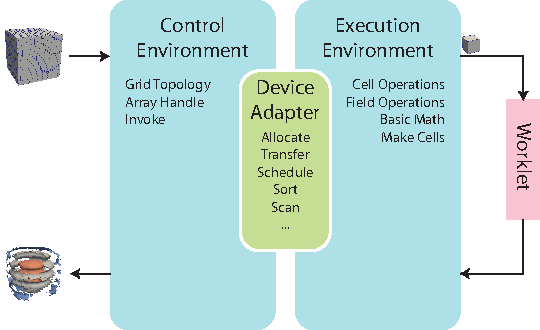
\includegraphics[width=\linewidth]{vtkm-framework}
  \caption{The basic VTK-m framework that allows device portability.}
  \label{fig:vtkm-framework}
\end{figure}
